\section{\textit{Nome do artigo}}


% ============================================================================
\subsection{Referência completa do artigo}

\begin{itemize}
  \item \textbf{Autores:} xxx
  \item \textbf{Local:} xxx
  \item \textbf{\textit{Journal}:} xxx [Qualis XXX]
  \item \textbf{Data:} xxx
  \item \textbf{Referência:} \citeonline{bib:2014:Autor}
\end{itemize}


% ============================================================================
\subsection{Resumo}
% ..........................................................
\subsubsection{Propósito do artigo}
xxx

% ..........................................................
\subsubsection{Técnicas utilizadas} 
% \begin{itemize}
%   \item xxx
% \end{itemize}  
xxx

% ..........................................................
\subsubsection{Contribuição em relação a artigos anteriores} %mais ou menos 10 linhas
% \begin{itemize}
%   \item xxx
% \end{itemize}  
xxx

% ============================================================================
\subsection{Metodologia}
% Descreva um pouco mais detalhadamente a metodologia e os resultados do artigo. 
% Inclua as figuras que achar mais relevantes.

Pra quem quiser citar colocando o nome do autor na frase é 
\citeonline{bib:2014:Autor} se quiser só se referenciar a ele é 
\cite{bib:2014:Autor}.

A Figura \ref{fig:2014:Autor:fig1} mostra uma cor feia! 

\begin{figure}[ht]
  \centering
  
\includegraphics[height=30px]{artigos/2014_Autor/fig1.png}
  \caption{Cor feia.}
  \label{fig:2014:Autor:fig1}
\end{figure}

A Equação \ref{eq:2014:Autor:soma} é uma soma:
\begin{equation}
  \label{eq:2014:Autor:soma}
  a (\mathbf{x}) = \sum^n_{i=1} x_i,
\end{equation}
onde $\mathbf{x}$ é um vetor.

Enquanto a Figura \ref{fig:2014:Autor:fig2} mostra uma cor linda! 

\begin{figure}[ht]
  \centering
  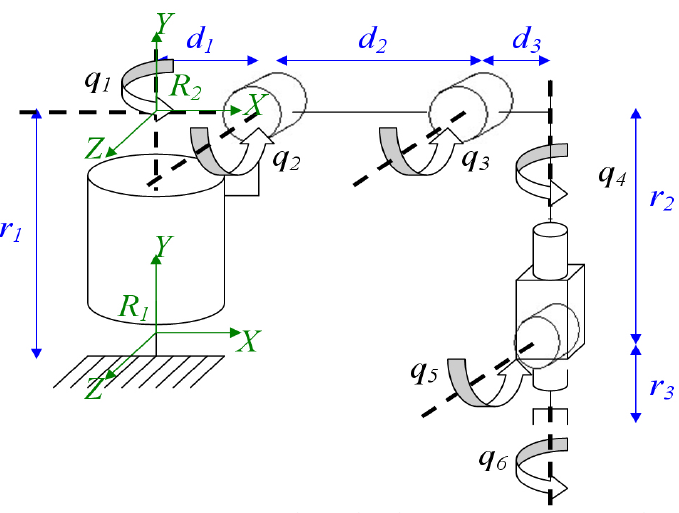
\includegraphics[height=100px]{artigos/2014_Autor/fig2.png}
  \caption{Cor bonita.}
  \label{fig:2014:Autor:fig2}
\end{figure}

% ..........................................................
\subsubsection{Resultados}
xxx

% ============================================================================
\subsection{Pontos fortes} %no máximo três
\begin{itemize}
  \item xxx
  \item xxx
  \item xxx
\end{itemize}  

% ============================================================================
\subsection{Limitações} %no máximo três
\begin{itemize}
  \item xxx
  \item xxx
  \item xxx
\end{itemize} 


% ============================================================================
\subsection{Avaliação}
\textbf{(a) Avanço considerável (\textit{Breakthrough}).}
% \textbf{(b) Contribuição significativa.}
% \textbf{(c) Contribuição modesta.}
% \textbf{(d) Contribuição fraca.}
% \textbf{(e) Sem contribuição.}
Justificativa.

% ============================================================================
\subsection{Problema em aberto}
% \begin{itemize}
%   \item xxx
% \end{itemize}  
xxx

% ============================================================================
\subsection{Aspecto obscuro}
% \begin{itemize}
%   \item xxx
% \end{itemize}  
xxx